\documentclass[12pt,a4paper]{article}
\usepackage[utf8]{inputenc}
\usepackage[english]{babel}
\usepackage{amsmath}
\usepackage{amsfonts}
\usepackage{amssymb}

\usepackage{hyperref}

\usepackage{graphicx}
\graphicspath{ {./images/} }
\usepackage{epstopdf}

\usepackage[top=1.5in, bottom=1in, left=1in, right=1in]{geometry}


% alignment of figures (H)
\usepackage{float}

% tikz graphs
\usepackage{tikz}
\usetikzlibrary{arrows,automata, positioning,calc,shapes.geometric}
\usepackage{varwidth} % for the diagram of fpga design

\usepackage{todonotes}

% for tanles
\usepackage{multirow}

% header
\usepackage{fancyhdr}
\pagestyle{fancyplain}
\fancyhf{}
\lhead{ \fancyplain{}{Lukas Schwartz \& Aitor Miguel } }
\rhead{ \fancyplain{}{EMB1 - 1. Semester MSc Robot Systems} }
\cfoot{ \fancyplain{}{\thepage} }

% make tables prettyer
\def\arraystretch{1.3}

\begin{document}

\begin{titlepage}
	\centering
%	\includegraphics[width=0.15\textwidth]{example-image-1x1}\par\vspace{1cm}
	\vfill
	{\scshape\LARGE University of Southern Denmark\par}
	\vspace{1cm}
	{\scshape\Large EMB1 Final Project\par}
	{\scshape\large 1. Semester MSc Robot Systems\par}
	\vspace{1.5cm}
	{\huge\bfseries Mini Segway\par}
	\vspace{2cm}
	{\Large\itshape Aitor Miguel Blanco \& Lukas Chr. M. W. Schwartz \\ Group \#1 \par}
	\vfill
	supervised by\par
	J\o rgen Christian Larsen \& Richard Beck

	\vspace{2cm}

% Bottom of the page
	{\large 23$^{rd}$ December 2015 \par}
\end{titlepage}

\pagebreak

\section*{Project Description}





what we need:

\begin{itemize}
\item 2 motors
\item accelerometer and gyroscope
\item FPGA (we have)
\item possibly ADC if analogue acc/gyro (we have)
\item motor driver (should be able to build ourself)
\end{itemize}

\pagebreak


\tableofcontents

\pagebreak

\listoffigures

\listoftables

\pagebreak


\section{Introduction}

In this project, the problem of solving automatically the sokoban game has been faced.
To do this, the project has been divided in two different parts, being studied separately.
These are finding the shortest solution given a sokoban map and the hardware implementation of a robot able to execute the generated path.

The system loads a map and finds a solution offline with a solver. 
The output of this program is a path that the robot should follow. 
This path is loaded onto the robot, which is prepared to execute it on the sokoban map.

The robot designed is made using different LEGO and LEGO Mindstorms parts and an NXT as controller.
And the solver is programmed using C++.

%The solver is based in the A* algorithm and implemented in C++.
\pagebreak


\section{Circuit and Physical Design}
To solve the sokoban problem a robot capable of performing simple tasks concerned with moving the can and itself around the game map are needed.
The behaviours the robot should be able to perform define how the robot should be formed in order to accomplish its task of solving the sokoban problem.


\subsection{Sensors}
In order to control and stabilize the Segway, then a set of sensors are required.
For this project it was decided to both use a set of sensors to control the systems stability and also to implement a set of sensors into the system enabling the tracking of the Segways position.


The tracking of the Segways position is done using an encoder kit\footnote{ \href{https://www.sparkfun.com/products/13339}{Wheel encoder}} mounted on the motors used in this project.
The encoders chosen for this project is an incremental rotary encoder capable to track the movement of the wheels, but not the direction of rotation.
It is hence not directly possible to tell which direction the Segway is moving without combining it with data from other sensors.
The sensors were however deemed good enough for the scope of this project.


The most important sensor of the system is the one used to control the stability of the system in order to hold it upright.
For this an accelerometer or/and a gyroscope can be used.
The advantage of using a gyroscope is that it is reliable in the measure of angular displacement over short periods of time.
When integrating over this it does, however, get troublesome due to drifts when performing the numerical integration.
The accelerometer on the other hand is exposed to a lot of noise from all the surrounding forces working on the system and it is hence only becomes a reliable measure of the systems angle when used with a low-pass filter.
It was therefore decided to use both in the project and combining them using a complimentary filter.
This provides the system with both the short term accuracy of the gyroscope and the long term reliability of the accelerometer.
For this project it was decided to by an integrated circuit
\footnote{ \href{https://www.sparkfun.com/products/13339}{IMU component}}
 including both gyroscope and accelerometer in the same component.
This ensures that the axis of the accelerometer and gyroscope are aligned within the component.





\subsection{Motor Control}
The motors chosen for this project were the two small geared DC motors\footnote{ \href{https://www.sparkfun.com/products/13258}{Motors}}.
In order to control them an H-bridge for both of the motors were constructed using the schematics in figure \ref{fig:hbridge}.


\begin{figure}[H]
\centering
%\includegraphics[width = 0.9 \textwidth]{•}

\caption{H-bridge schematics.}
\label{fig:hbridge}
\end{figure}

A full H-bridge is required in order to control the Segways movement in both directions such that it is able to both move and recover from a fall when moving around.
Each motor is made with each their separate H-bridge in order to facilitate the rotation of the segway.

\todo[inline]{write short about the h bridge design and different transistors used}


\subsection{The Segway System}
The segway was constructed using a metal plate as foundation for the robot.
The motors were then attached to the lower side of the plate.
On top of the basis was then mounted the PCB designed with the two H-bridges to control the two motors.

A second layer was then added as a plug-in module to which the different components could be plugged in and on which the power supply circuit is, converting the input voltage to a 5V supply for the FPGA.
This layer included a plug for the FPGA and the IMU.
Furthermore was there added plugs for a bluetooth sender/transmitter and two wheel encoders, but due to time constraints was it chosen not to use their functionality since it was not required for the system to work at the given state.

A sketch of the final segway is seen in figure \ref{fig:segwaysketch}.

\begin{figure}[H]
\centering
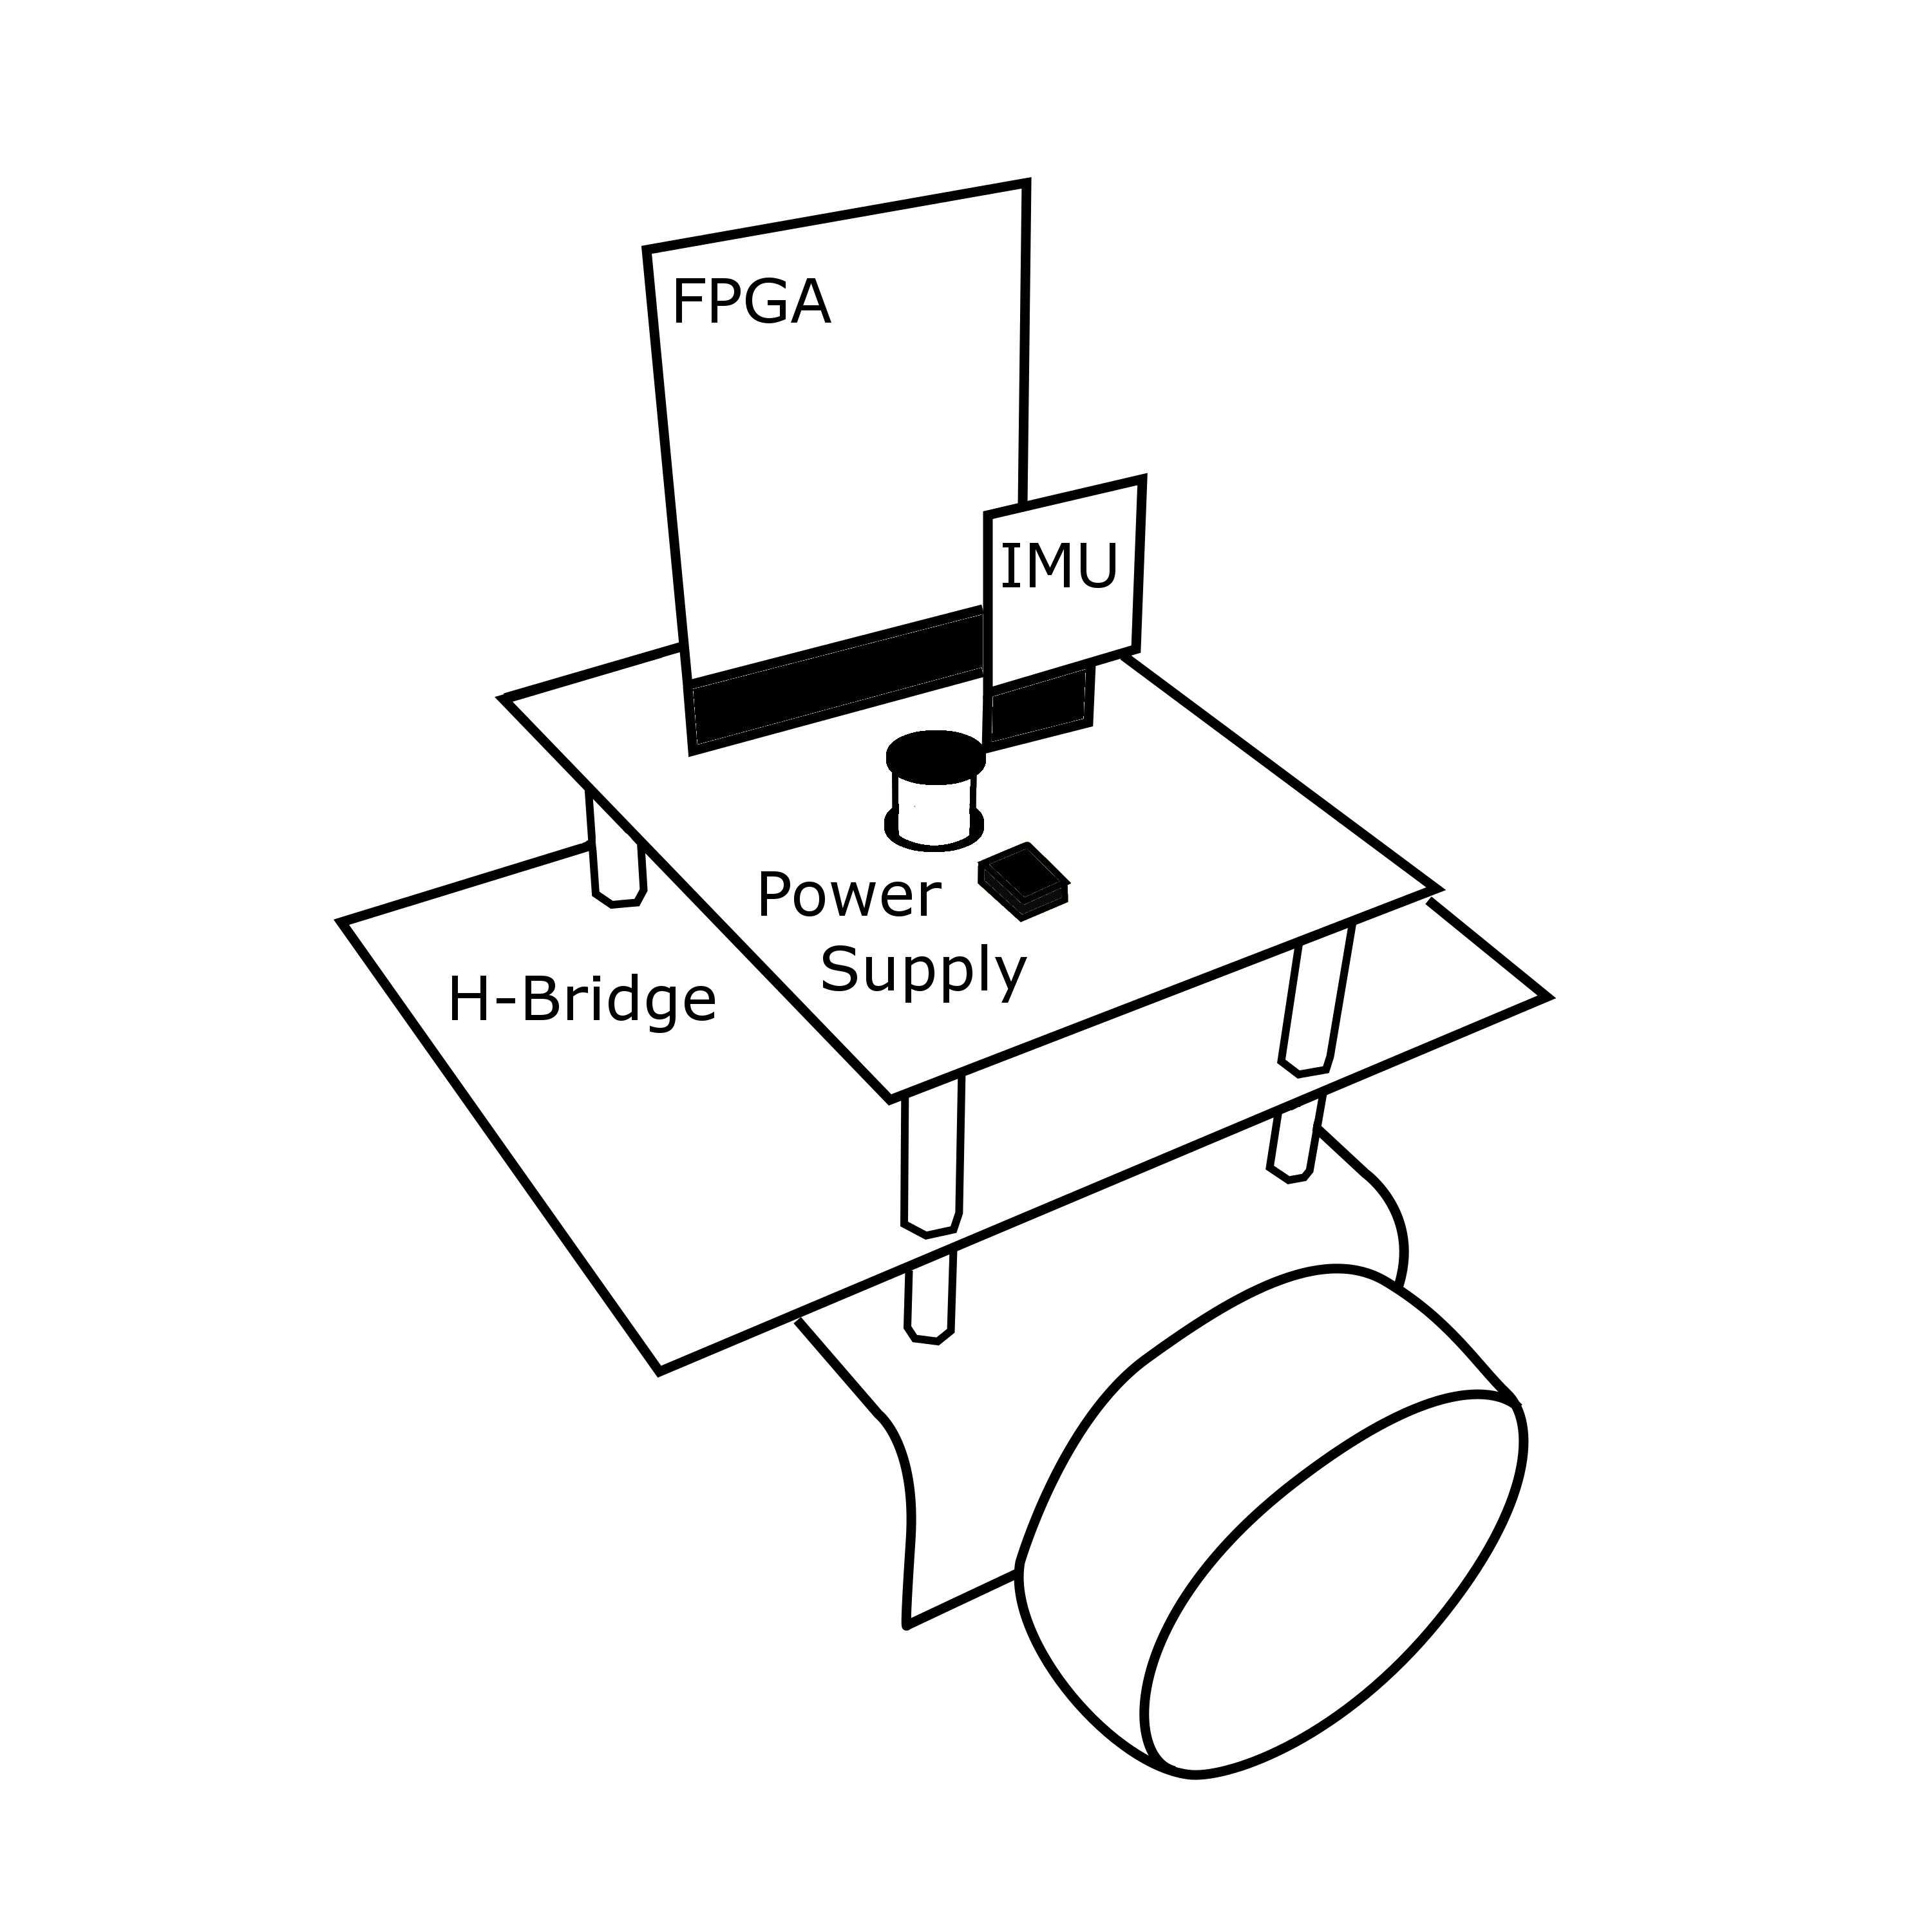
\includegraphics[width = 0.5 \textwidth]{images/segway}
\caption{Sketch of the build segway.}
\label{fig:segwaysketch}
\end{figure}

As seen on figure \ref{fig:segwaysketch}, then the goal of the final segway design was to center the center of mass above the wheel axis when the segway stands in upright position.
This was done by using mirrored design, where possible, when designing the boards and center the FPGA and other electronics about the same axis.


\subsection{Conclusion}


\pagebreak
\section{Software}
In order to control and stabilize the segway a the communication with the accelerometer/gyroscope must be established.
This must data received must then be processed in order to control the motors according to the segways position.



\begin{figure}[H]
\centering

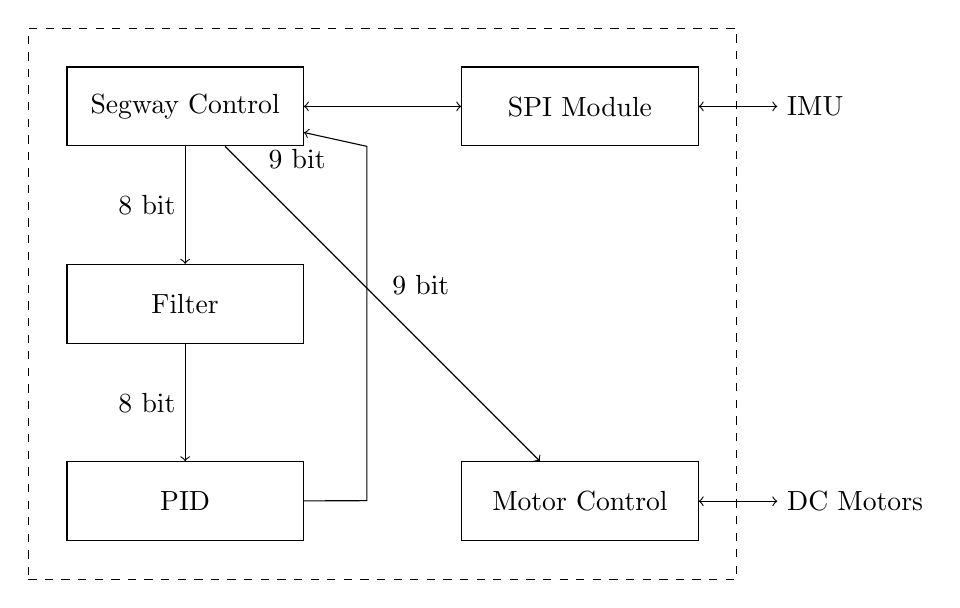
\begin{tikzpicture}[node distance=1cm]
% FPGA border
\node[rectangle,draw,minimum width=9cm, minimum height=7cm, dashed, name=FPGA]  {};

% used to align the insides of FPGA
\node[rectangle,minimum width=5cm, minimum height=5cm, name=FPGAaligne] {};

% components of FPGA
\node[rectangle,draw,minimum width=3cm, minimum height=1cm, name=pid] at (FPGAaligne.-135) {PID};
\node[rectangle,draw,minimum width=3cm, minimum height=1cm, name=communiction] at (FPGAaligne.45) {SPI Module};
\node[rectangle,draw,minimum width=3cm, minimum height=1cm, name=mc] at (FPGAaligne.-45) {Motor Control};
\node[rectangle,draw,minimum width=3cm, minimum height=1cm, name=filter] at (FPGAaligne.180) {Filter};
\node[rectangle,draw,minimum width=3cm, minimum height=1cm, name=segway] at (FPGAaligne.135) {Segway Control};

% nodes outside FPGA
%\node [left=of utos,name=pc] {PC};
\node [right=of communiction,name=spi] {IMU};
%\node [left=of color,name=rgb] {RGB(2:0)};
\node [right=of mc,name=motor] {DC Motors};

% arrows inside FPGA
\draw[<->] (segway) -- node[] {} (communiction) ;
\draw[->] (segway) -- node[left] {8 bit} (filter) ;
\draw[->] (filter) --  node[left] {8 bit} (pid) ;
\draw[->] (segway) -- node[above right] {9 bit} (mc) ;
\draw[->] (pid) --(-0.2,-2.5)--(-0.2,2)-- node[below left] {9 bit} (segway) ;
 
% arrows connected to the outside of FPGA
\draw[<->] (spi) -- node[] {} (communiction) ;
\draw[<->] (mc) -- node[] {} (motor) ;
%\draw[->] (adc) to[out=180, in=0] node[] {} (ad) ;
%\draw[->] (color) to[out=180, in=0] node[] {} (rgb) ;
%\draw[->] (mc) to[out=0, in=180] node[] {} (servo) ;
\end{tikzpicture}

\caption{Block design of the FPGA.}
\label{fig:fpga_sof_design}
\end{figure}


The designed system is comprised by the modules seen in figure \ref{fig:fpga_sof_design}.
Here the \textit{Segway Control} block is the main part of the system, used to combine the different components into one.
The \textit{SPI Module} takes care of the communication with the accelerometer and gyroscope by sending data to such when asked for by the \textit{Segway Control} module.

Data from such is then send to the \textit{Filter} to predict an angle.
From here the angle is passed to the \textit{PID} in order to generate a duty cycle which is then passed back to the main module, the \textit{Segway Control}.
The \textit{Segway Control} hence also takes care to set the right ports on the H-bridges, through the \textit{Motor Control} unit, depending on the speed and direction bit generated by the \textit{PID}.
The five components are explained further throughout this section.

\subsection{Segway Control}
The segway control module is the top module of the design and in charge of the data transfer between the different underlying modules and the communication with the IMU.
It is implemented as the state machine seen in figure \ref{fig:segwaycontrol_fsm}.


\begin{figure}[H]
\centering

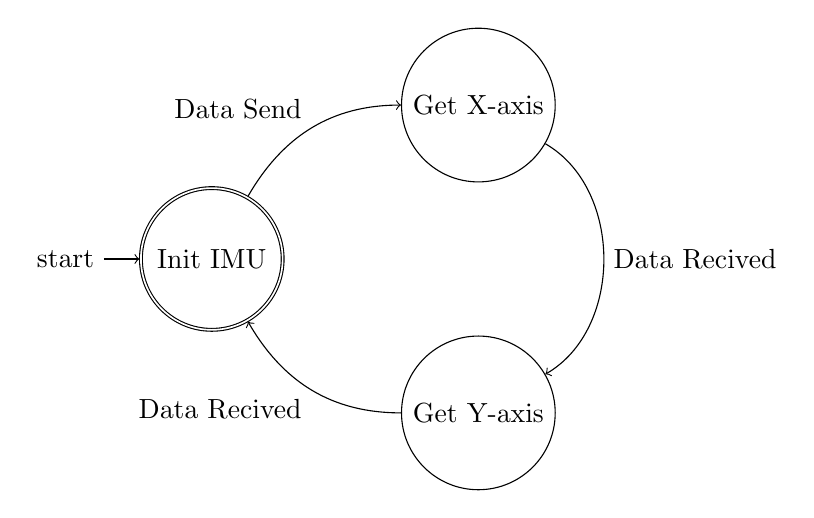
\begin{tikzpicture}[node distance=3cm]
\node[circle, minimum width=4.5cm, name=c] {};

% node circles
\node[initial,accepting,state,name=init,minimum width=1.8cm] at (c.180)   {Init IMU}; 
\node[state,name=xaxis,minimum width=1.8cm] at (c.60)   {Get X-axis}; 
\node[state,name=yaxis,minimum width=1.8cm] at (c.-60)   {Get Y-axis}; 

% connections
\draw[->] (init) to[out=60, in=180] node[midway,above left] {Data Send} (xaxis) ;
\draw[->] (xaxis) to[out=-30, in=30] node[midway,right] {Data Recived} (yaxis) ;
\draw[->] (yaxis) to[out=-180, in=-60] node[midway,below left] {Data Recived} (init) ;
 
\end{tikzpicture}

\caption{Finite state machine of the Segway Control module.}
\label{fig:segwaycontrol_fsm}
\end{figure}

The module is, as seen in figure \ref{fig:segwaycontrol_fsm}, looping between a set of states where it is communicating with the IMU.
In the current design only acceleration of the robot in the frontal/backward direction (x-axis) is considered, as explained in section \ref{sec:controlproblem}.
This is hence the only value stored and send onwards in the system.
The values of interest are requested in the state machine and then send to the \textit{filter} module for further processing.

In the state machine seen, the IMU is initiated every cycle.
This was done to ensure that the IMU is configured correctly when data is requested due to the possibility that a short power break shuts down the IMU and forces it into its default sleep mode.


\subsection{SPI Module}
To communicate with the IMU a SPI module was made.
The module is made up of three phases.
One being the phase where the slave is told what is going to happen.
The second being the read or write phase where the FPGA either reads data from the IMU or sends data to the IMU.
Finally there is the wait state where there is no communication amongst the two units.

The SPI module was implemented as an 8 bit data transmitter and receiver.
It is however possible to read multiple bytes in succession from the IMU, it was however deemed unnecessary to use all 16 bit the current version of the segway.
\subsection{Data Filter}

The value in an accelerometer is often noisy.
In our case the noise largely originates from motor vibrations and the acceleration caused by the general movement of the segway.
This can give problems in cases where small movements of the device are important and in general if big noise spikes are encountered.
To solve this problem, the commonly used solution is to combine the value given by the gyroscope with that of the accelerometer readings to obtain a more accurate prediction of the angle.
As this approach is complex and not really needed to obtain a simple control of the segway, a more simple solution was selected.

The accelerometer data is filtered using a mean filter to reduce high frequency noise form the motor vibrations.
The filtering module calculates the mean of the last eight readings from the accelerometer, giving as an output a 8 bit value.
This 8 bits represent the value of acceleration obtained, being 0 m/s$^{2}$ the value 127, all the values above it positive and all the values below negative.
This filter module is also used to converter the data from the accelerometers format into this new data representation going from negative acceleration at 0 to positive acceleration at 256 and zero acceleration at 127.
\subsection{PID Controller}

The PID module developed implements a PID controller using as a input a reference signal for the desired value of the accelerometer and the actual acceleration value as two logic vectors.

As all the operations in the PID are calculated using integers, then the data vectors are converted into integers before the operations and reconverted into a logic vector afterwards.
%The  again representing the value of the duty cycle needed in the motors and their direction.
The output vector generated is a 9 bit signal.
The eight least significant bits representing the chosen duty cycle and the most significant bit the direction of the motors, that is positive for forward and negative backwards.

Three different values can then be set to modify the PID performance.
The gain for the proportional, integral and differential part.

\subsection{Motor Control}
The Motor control unit controls the input to the eight different inputs on the two H-bridges.
This control was implemented as the finite state machine seen in figure \ref{fig:motorcontrol_fsm}.

The main purpose of the motor control unit is to set two of the ports of the motor low and the two others high depending on the direction the segway is moving.
When controlling the speed a PWM signal is send to one of the ports of the H-bridge to control the speed depending on the value calculated in the PID controller.


\begin{figure}[H]
\centering

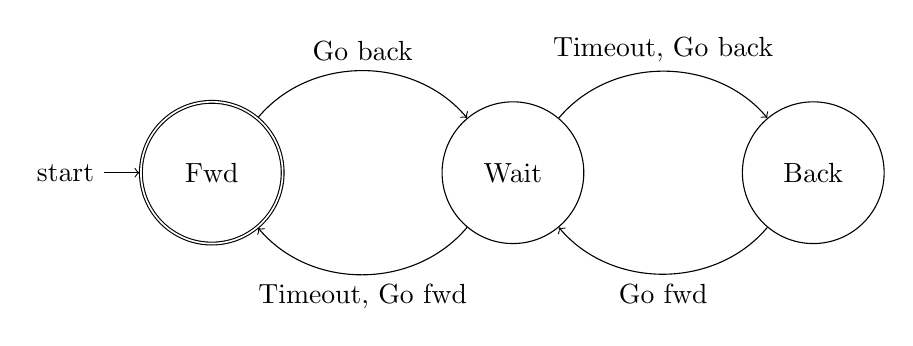
\begin{tikzpicture}[node distance=2cm]

% node circles
\node[initial,accepting,state,name=fwd,minimum width=1.8cm] {Fwd}; 
\node[state,name=wait,minimum width=1.8cm, right=of fwd] {Wait}; 
\node[state,name=back,minimum width=1.8cm, right=of wait] {Back}; 

% connections
\draw[->] (fwd) to[out=50, in=130] node[midway,above] {Go back} (wait) ;
\draw[->] (wait) to[out=50, in=130] node[midway,above] {Timeout, Go back} (back) ;
\draw[<-] (fwd) to[out=-50, in=-130] node[midway,below] {Timeout, Go fwd} (wait) ;
\draw[<-] (wait) to[out=-50, in=-130] node[midway,below] {Go fwd} (back) ;
 
\end{tikzpicture}

\caption{Finite state machine of the Motor Control module.}
\label{fig:motorcontrol_fsm}
\end{figure}


As seen on figure \ref{fig:motorcontrol_fsm}, then a wait state is put between the two driving states, forward and backward.
This was done to protect the motor when switching between the states.
It is necessary to have a delay because of the turn of and turn on delays of the transistors.
If this is not set it may result in all the transistors being open at once and thus damaging the motor.
The delay was set to 160ns which is considerably more than the turn on and turn of delay of the transistors, but small enough that it should not be noticed when driving the motors.
During this time all the transistors are set off.

The PWM generated at the motors is based on a 8 bit signal and there are hence 256 different duty cycles to drive the motors with.

\subsection{Conclusion}
An A* algorithm was devised to solve the Sokoban problem.
The algorithm uses a graph structure where the nodes represent diamond pushes with the cost being the number of steps the robot must move in order to achieve the state.

The heuristic for the A* algorithm was found calculating the cost for the robot to move each diamond from their current position to the nearest goal.
This technique takes into account the walls on the map, but disregard the diamonds left on the map disrupting the path.
Furthermore the cost of moving in between the diamonds and the fact that one goal may be considered the destination of multiple diamonds is not taken into account using this method.

The nodes in the graph where also validated using their state, in form of the diamonds and robots position, as the key in a hashing table.
Furthermore the states are checked for simple deadlock situations.





\pagebreak
\section{Test of the System}
The final system was tested to see how well it performs.
The tests where performed in a set of different lighting conditions and with the thresholds set beforehand to a suitable value.

The first set of test where conducted with thresholds tuned to work in approximate normal ambient lighting and hereafter the same set of tests where conducted with new thresholds trying to make them work in all conditions.


\subsection{Test One: Thresholds for Normal Ambient Lighting}

The thresholds for the color detector were first tuned using the values read from the FPGA under normal lighting conditions.
These thresholds for the red, green and blue brick colors were then used in the experiment.

The three different bricks were let slide through the setup and the result shown in the confusion tables in table \ref{tab:confusiontable_testresults_01_normal}, \ref{tab:confusiontable_testresults_01_low}, \ref{tab:confusiontable_testresults_01_direct} and \ref{tab:confusiontable_testresults_01_high} for the light levels normal and low lighting, lighting directly into the photodiode and strong lighting from the side respectively.


\begin{table}[H]
\centering
\begin{tabular}{c c|c|c|c|c|}
\cline{3-6}
 & &  \multicolumn{4}{|c|}{Predicted} \\ \cline{3-6}
 & & Red & Green & Blue & None \\ \cline{1-6} 
\multicolumn{1}{ |c|  }{\multirow{3}{*}{Actual}} & Red & 19 & 0 & 0 & 1 \\ \cline{2-6}
\multicolumn{1}{ |c|  }{} & Green & 0 & 20 & 0 & 0 \\ \cline{2-6}
\multicolumn{1}{ |c|  }{} & Blue & 0 & 0 & 20 & 0 \\ \hline
\end{tabular}
\caption[Confusion table in normal ambient lightning, test one.]{Confusion table of the test results in normal ambient lightning using thresholds tuned for normal ambient lighting.}
\label{tab:confusiontable_testresults_01_normal}
\end{table}



\begin{table}[H]
\centering
\begin{tabular}{c c|c|c|c|c|}
\cline{3-6}
 & &  \multicolumn{4}{|c|}{Predicted} \\ \cline{3-6}
 & & Red & Green & Blue & None \\ \cline{1-6} 
\multicolumn{1}{ |c|  }{\multirow{3}{*}{Actual}} & Red & 9 & 0 & 0 & 11 \\ \cline{2-6}
\multicolumn{1}{ |c|  }{} & Green & 0 & 13 & 0 & 7 \\ \cline{2-6}
\multicolumn{1}{ |c|  }{} & Blue & 0 & 0 & 20 & 0 \\ \hline
\end{tabular}
\caption[Confusion table in normal low lightning, test one.]{Confusion table of the test results in a dark/low lit room using thresholds tuned for  normal ambient lighting.}
\label{tab:confusiontable_testresults_01_low}
\end{table}


\begin{table}[H]
\centering
\begin{tabular}{c c|c|c|c|c|}
\cline{3-6}
 & &  \multicolumn{4}{|c|}{Predicted} \\ \cline{3-6}
 & & Red & Green & Blue & None \\ \cline{1-6} 
\multicolumn{1}{ |c|  }{\multirow{3}{*}{Actual}} & Red & 0 & 0 & 0 & 20 \\ \cline{2-6}
\multicolumn{1}{ |c|  }{} & Green & 0 & 0 & 0 & 20 \\ \cline{2-6}
\multicolumn{1}{ |c|  }{} & Blue & 0 & 0 & 0 & 20 \\ \hline
\end{tabular}
\caption[Confusion table in high ambient lightning, test one.]{Confusion table of the test results in high ambient lightning where there is lit directly into the photodiode using thresholds tuned for  normal ambient lighting.}
\label{tab:confusiontable_testresults_01_direct}
\end{table}


\begin{table}[H]
\centering
\begin{tabular}{c c|c|c|c|c|}
\cline{3-6}
 & &  \multicolumn{4}{|c|}{Predicted} \\ \cline{3-6}
 & & Red & Green & Blue & None \\ \cline{1-6} 
\multicolumn{1}{ |c|  }{\multirow{3}{*}{Actual}} & Red & 10 & 0 & 0 & 10 \\ \cline{2-6}
\multicolumn{1}{ |c|  }{} & Green & 0 & 10 & 0 & 10 \\ \cline{2-6}
\multicolumn{1}{ |c|  }{} & Blue & 0 & 0 & 11 & 9 \\ \hline
\end{tabular}
\caption[Confusion table in high ambient lightning, test one.]{Confusion table of the test results in high ambient lighting with no lighting directly into the photodiode using thresholds tuned for  normal ambient lighting.}
\label{tab:confusiontable_testresults_01_high}
\end{table}


It was during these test found that the sorter correctly sorted 59 out of the 60 bricks in normal lighting.
But when used in different lighting setups, this went down to 31/60 when in strong lighting and 42/60 when in low lighting.
And when the sensor is directly exposed to a light source it is able to detect nothing.

This is expected to happen since the thresholds are only found by looking at the values for normal lighting conditions and a naive approach is used were  it is always expected that the brick gives the same response no matter the lighting.

In order to improve these results a set of new experiments were conducted with new thresholds based on the values obtained from the sensor in the other lighting conditions as well.
This is seen in section \ref{sec:testtwo}.



\subsection{Test Two: Thresholds for Larger Spectrum of Lighting Conditions}
\label{sec:testtwo}

The second test was conducted the same way as the previous, but with a new set of thresholds defined depending on the light intensity when the surroundings have different lighting levels.

This resulted in the confusion tables in table \ref{tab:confusiontable_testresults_02_low}, \ref{tab:confusiontable_testresults_02_direct} and \ref{tab:confusiontable_testresults_02_high} for the light levels low lighting, lighting directly into the photodiode and strong lighting from the side respectively.
Tests were also tried to be conducted at normal lighting, but this failed due to the system detecting colors randomly due to the reflections of the slide and other surroundings.


% normal ambient lighting failed...

\begin{table}[H]
\centering
\begin{tabular}{c c|c|c|c|c|}
\cline{3-6}
 & &  \multicolumn{4}{|c|}{Predicted} \\ \cline{3-6}
 & & Red & Green & Blue & None \\ \cline{1-6} 
\multicolumn{1}{ |c|  }{\multirow{3}{*}{Actual}} & Red & 20 & 0 & 0 & 0 \\ \cline{2-6}
\multicolumn{1}{ |c|  }{} & Green & 0 & 20 & 0 & 0 \\ \cline{2-6}
\multicolumn{1}{ |c|  }{} & Blue & 0 & 1 & 19 & 0 \\ \hline
\end{tabular}
\caption[Confusion table in low lightning, test two.]{Confusion table of the test results in a dark/low lit room using thresholds tuned for larger spectrum of lighting conditions.}
\label{tab:confusiontable_testresults_02_low}
\end{table}


\begin{table}[H]
\centering
\begin{tabular}{c c|c|c|c|c|}
\cline{3-6}
 & &  \multicolumn{4}{|c|}{Predicted} \\ \cline{3-6}
 & & Red & Green & Blue & None \\ \cline{1-6} 
\multicolumn{1}{ |c|  }{\multirow{3}{*}{Actual}} & Red & 19 & 0 & 0 & 1 \\ \cline{2-6}
\multicolumn{1}{ |c|  }{} & Green & 0 & 20 & 0 & 0 \\ \cline{2-6}
\multicolumn{1}{ |c|  }{} & Blue & 0 & 10 & 10 & 0 \\ \hline
\end{tabular}
\caption[Confusion table in high ambient lightning, test two.]{Confusion table of the test results in high ambient lightning where there is lit directly into the photodiode using thresholds tuned for larger spectrum of lighting conditions.}
\label{tab:confusiontable_testresults_02_direct}
\end{table}


\begin{table}[H]
\centering
\begin{tabular}{c c|c|c|c|c|}
\cline{3-6}
 & &  \multicolumn{4}{|c|}{Predicted} \\ \cline{3-6}
 & & Red & Green & Blue & None \\ \cline{1-6} 
\multicolumn{1}{ |c|  }{\multirow{3}{*}{Actual}} & Red & 20 & 0 & 0 & 0 \\ \cline{2-6}
\multicolumn{1}{ |c|  }{} & Green & 0 & 0 & 20 & 0 \\ \cline{2-6}
\multicolumn{1}{ |c|  }{} & Blue & 0 & 0 & 20 & 0 \\ \hline
\end{tabular}
\caption[Confusion table in high ambient lightning, test two.]{Confusion table of the test results in high ambient lighting with no lighting directly into the photodiode using thresholds tuned for larger spectrum of lighting conditions.}
\label{tab:confusiontable_testresults_02_high}
\end{table}


It can be seen that the brick sorter performs considerably better in low lit conditions where its correct detection rate is 59/60.
Likewise it is able to detect 49/60 correct when light it lit directly into the photodiode where 10 of the errors are misclassification.
The setup is however detecting green bricks as blue when there is higher ambient lighting whereas it always detects the red and blue correctly.

It can therefore be concluded that the used thresholds are only suitable for low lit conditions and overall gives worse results when considering that it is not able to detect anything in normal conditions.



\subsection{Test Analysis}

% the method used to detect color algorithm is NOT invariant of ambient lighting.
The two tests preformed were both using a set of fixed thresholds for which each color has to lie within, in order to be detected as a brick of that color.
That is a brick needs to consist of a limited range of red, green and blue color.
This is a method that is not invariant to the lighting conditions.
The used method was, however chosen because of its ease of implementation.

It is therefore expected that it should be possible to improve the results of the brick sorter by using a ambient light-level invariant, or at least semi-invariant, method for detection.
These methods can be based both on the ratio of the colors, rather than the level.
Furthermore it is possible to include the use of the ambient light-level when no LED is on.
This should, by taken the difference between when the LEDs are on and when not, give a result capable of handling more noise in form of changes in the lighting.

One problem does however also arises when the color detection method is invariant to the lighting level.
That is the photodiods signal going in saturation because of complete over lighting because the amplification of the diode is only designed to work within a specific range.
This would in most cases cause problems if all the three colors reach saturation as one can then not distinguish between the levels.
A possible way of solving this problem can be made by a change in hardware.
By introducing different amplifications on the photodiode, a set of ranges can then be used such that the amplification is lower when the setup is used in higher lighting settings and vice versa.
The final implementation of such a circuit could be to have multiple amplifier circuits connected to different input ports on the ADC.
The FPGA can then sample from the port that gives the best overall resolution on the three color intensities.

The used implementation can also be improved by changing the physical properties of the slide.
By building a dark cage around the color detecting circuit, it should be possible to hold the light level around the detector more or less constant.
Thus improving the systems robustness to the light changes around it.




\subsection{Conclusion}
Tests were conducted to test the functionality of the system when using fixed thresholds.
It was found that this worked sufficiently (almost 100\% accuracy) in cases were the ambient lighting is fixed, but less so in environments with changing lighting.

The results were hence analysed and a set of changes to both the physical and software system was suggested to improve the performance by making the system invariant to changes in lighting.








\pagebreak
\section{Conclusion}



\pagebreak
\section{Discussion}
The segway constructed has a physical design of such that it is deemed good enough.
The only changes which should be made are replacements of the connectors which should be updated to give a more reliable connection to the motors and from the power supply to the H-bridge.

Since the system was not able to balance itself, then it is probably the software system that is needing the biggest upgrade.
This includes going away from only using only one axis of the accelerometer and trying to set its the gravitational effect of such to zero.
To possibly using two axis of the accelerometer to predict the actual angle of the segway.
This would require the implementation of the 'atan' function on the FPGA.
Given that the current FPGA used only has 54k bits of block RAM, then this implementation has to be an approximation of the function since not enough space is present for a direct table lookup.

Given that a successful implementation of the calculation of the angle of the segway has been found, then this can also be combined with the gyroscope data.
This can then be used to implement a complimentary filter, Kalman filter or similar.

It is furthermore possible to investigating other controller options to improve the performance of the segway or use different controllers when in different situations.
That is having different PID controllers when the segways incline is within a certain range.

Once the segway is able to stand by itself it would also be of interest to make it possible to control it through the bluetooth device.
The encoders could then be used to control its odometry of the segway to turn it and drive it around a specific speeds.

\pagebreak
\appendix




\end{document}